\begin{answer}\\
Lets look at the plots for both datasets after 30,000 iterations (since we have convergence for dataset A soon after)\\
\begin{figure}
  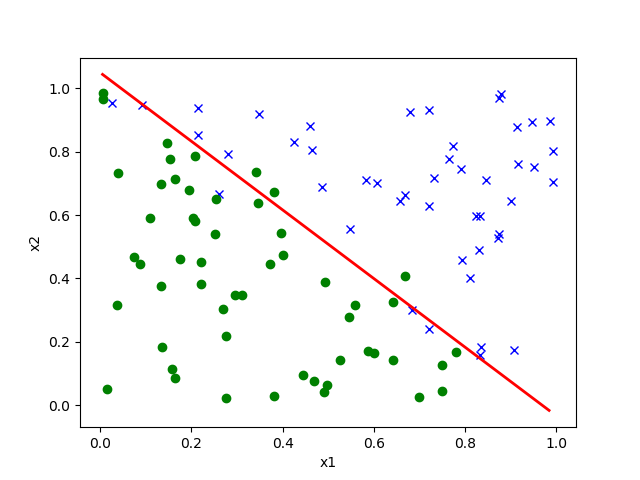
\includegraphics[width=\linewidth]{../src/output/A_30000.png}
  \caption{Dateset A with decision boundary after 30,000 iterations}
  \label{fig:Dateset A with decision boundary after 30,000 iterations}
\end{figure}\\
\begin{figure}
  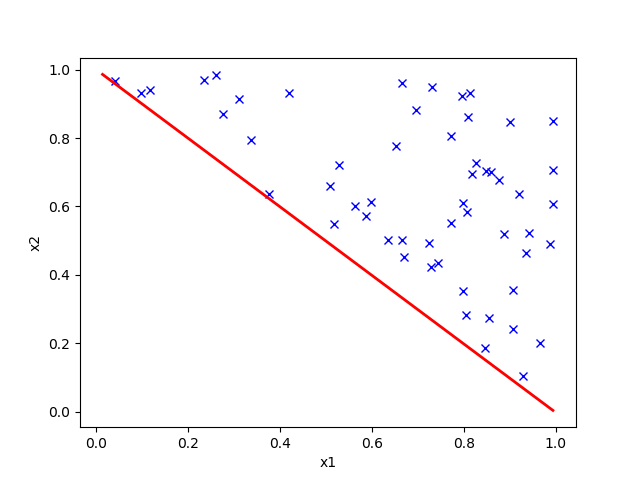
\includegraphics[width=\linewidth]{../src/output/B_30000.png}
  \caption{Dateset B with decision boundary after 30,000 iterations}
  \label{fig:Dateset B with decision boundary after 30,000 iterations}
\end{figure}\\
We see that dataset B is perfectly linearly separable. Recall that we are trying to find a $\theta$ s.t. we maximize the likelihood which is given by\\
$L(\theta)=\prod_{i=1}^{m}p(Y=y^{(i)}|x^{(i)};\theta)=\prod_{i=1}^{m}\frac{1}{1+e^{-y^{(i)}(x^{(i)})^T \theta}}$\\
The larger the value of $y^{(i)}(x^{(i)})^T \theta$, the higher the value of $L(\theta)$. But in the case of dataset B, we can keep increasing $\theta$ to get a higher likelihood.\\
In fact, as $\theta \rightarrow \infty, L(\theta) \rightarrow max$.\\
Thats why the dataset $B$ does not converge.
\end{answer}
